\documentclass[dvipdfmx,uplatex]{jsarticle}
\usepackage{tosuustd2019}
\newtheorem{claimindep}{主張}

\title{閉曲面の分類定理}
\author{みつば(@mittlear1)}
\date{2019年6月29日}

\begin{document}
\maketitle
\section{イントロダクション}
「マグカップと浮き輪は同じ形をしている」と主張されることがある.しかし,両者は合同ではないから同じ図形ではないと主張することもできる.このように,与えられた二つの図形が同じかどうかということはそれを判断するための基準がないと回答することができない問いである.「合同」という視点から見ると確かに両者は異なる図形だが,「一方を変形させて他方に移すことができるか」という視点では両者は同じ図形であると言うことができる.

高校数学でも,図形を比較するための基準として合同を用いることもあれば相似を用いることもあった.他にも角がいくつあるかで図形を分類することもできるだろう.「$n$角形の内角の和が$(n-2)\pi$である」という定理は,この基準において幾何学を考えたときの定理であると言うことができる.普段はこのような「基準」の違いを意識することはないかもしれないが,これによってものごとの本質をとらえやすくなったり,状況をうまく整理できるようになったりすることがある.

今回はその基準として「同相」と呼ばれるものを用いる.これは一番初めに例示したような「マグカップと浮き輪を同一視する」幾何学である.
\begin{definition}\label{homeo}
二つの位相空間$X$, $Y$が同相であるとは,連続写像$\map{f}{X}{Y}$と$\map{g}{Y}{X}$が存在し,$g\circ f=\id_X$, $f\circ g=\id_Y$をみたすことをいう.
\end{definition}

平たく言えば,図形のつながり具合が同じ図形たちを同じと見なすような基準が同相である.

\begin{example}
同相な図形の例を挙げる.
\begin{enumromanp}
\item 直線と曲線.
\item 三角形の周と円周.
\item トーラス(浮き輪)とマグカップ.
\end{enumromanp}
同相でない図形の例を挙げる.
\begin{enumromanp}
\item 一つの直線と二つの直線.
\item 一つの直線と三角形.
\item 球面とトーラス.
\end{enumromanp}
\end{example}

\begin{remark}
定義\ref{homeo}のように同じであるための基準を定めたとしても,トーラスとマグカップが同じであることを示すのはやはり難しい.なぜなら,トーラスとマグカップを数学の言葉で書く(例えばパラメータ付けをするなど)必要があるからである.

また,二つの図形が同相でないことの証明は同相であることの証明に比べてずっと難しい.同相であることの証明はうまい写像を作ればいいのに対して,同相でないことの証明はそのような写像が絶対にないことを示さないといけないからである.同相でないことの証明には,しばしば同相な図形の間で変わらない量(位相不変量)が使われる.
\end{remark}

高校数学までで扱ってきたような,「合同」を図形の比較の基準として用いる幾何学はEuclid幾何学と呼ばれる.対して「同相(あるいはホモトピー同値)」を図形の同一視の基準として用いる数学の一分野をトポロジー(位相幾何学)という.

\begin{remark}
「同じ」であることの基準を定めるということは幾何学に限らず,数学全体に通底するテーマである.例えば線型代数なら線型同型が,群論なら群同型が「同じ」であることの基準である.数学の多くの分野は,「数学的対象とそれらの同一視の基準」という構造を持っている.これらの概念を抽象化して調べる分野に圏論がある.
\end{remark}

本稿で扱う図形は閉曲面とよばれるものである.閉曲面とは,無限の広がりを持たず,さらにふちを持たない図形のことである.例えば2次元平面全体は無限の広がりを持つので今回の考察の対象ではない.お椀の形をした図形は無限の広がりを持たないがふちを持つので閉曲面ではない.一方,球の表面や浮き輪は閉曲面の代表的な例である.

2次元平面すら排除されてしまうような図形たちしか扱わないのだからそんなに種類がない気がしてしまうかもしれないが,実際にどのくらいあるのかを調べるのは簡単な問題ではない.この問題に解答を与えるのが今回の目標である.

\section{閉曲面の定義}
まずは閉曲面という概念に正確な定義を与える.

\begin{definition}
$r\geq 2$とする.境界が$r$個の点によって分割された2次元円板を位相的$r$角形という.
\end{definition}

$r\geq 3$のとき位相的$r$角形は凸$r$角形と同一視できる.

$P_1,\dots , P_n$を位相的多角形とする.さらに多角形のどの辺も他の一つの辺とペアになっていて,そのペアの間には同相写像が与えられているとする.この多角形たちと同相写像の組を多角形系とよぶ.多角形系を一つの文字$\mscrP$で表す.

\begin{definition}\label{surface}
多角形系$\mscrP$が与えられたとき,各辺を与えられた同相写像によって貼りつけてできる空間を$\mscrP$の実現といい,$\abs{\mscrP}$と書く.位相空間$X$がある多角形系$\mscrP$の実現と同相になるとき,$X$は閉曲面であるという.
\end{definition}

\begin{example}\label{eg surface}
閉曲面の例をいくつか挙げる.以下の例では,同じマークをつけた辺を向きをそろえて貼りつける.
\begin{enumarabicp}
\item 2次元球面.
\begin{center}
\begin{tikzpicture}
  \draw  (0,0) -- (4,0);
  \draw  (0,0) -- (2,3.4);
  \draw  (4,0) -- (2,3.4); %左側の正三角形
  \draw[line width=0.3mm]  (1.1,1.87) -- (0.8,1.65);
  \draw[line width=0.3mm]  (1.1,1.87) -- (1.05,1.5); %左の矢印
  \draw[line width=0.3mm]  (2.,0) -- (1.7,0.15);
  \draw[line width=0.3mm]  (2,0) -- (1.7,-0.15); %下の矢印
  \draw[line width=0.3mm]  (2.1,-0.15) -- (2.1,0.15); %下の縦棒
  \draw[line width=0.3mm]  (2.8,2.04) -- (3.1,1.82);
  \draw[line width=0.3mm]  (2.8,2.04) -- (2.85,1.67); %右上の矢印
  \draw[line width=0.3mm]  (3.0,1.7) -- (3.3,1.48);
  \draw[line width=0.3mm]  (3.0,1.7) -- (3.05,1.33); %右下の矢印

  \draw  (7,0) -- (11,0);
 \draw  (0,0) -- (4,0);
  \draw  (7,0) -- (9,3.4);
  \draw  (11,0) -- (9,3.4); %右側の正三角形
  \draw[line width=0.3mm]  (8.1,1.87) -- (7.8,1.65);
  \draw[line width=0.3mm]  (8.1,1.87) -- (8.05,1.5); %左の矢印
  \draw[line width=0.3mm]  (9.,0) -- (8.7,0.15);
  \draw[line width=0.3mm]  (9,0) -- (8.7,-0.15); %下の矢印
  \draw[line width=0.3mm]  (9.1,-0.15) -- (9.1,0.15); %下の縦棒
  \draw[line width=0.3mm]  (9.8,2.04) -- (10.1,1.82);
  \draw[line width=0.3mm]  (9.8,2.04) -- (9.85,1.67); %右上の矢印
  \draw[line width=0.3mm]  (10.0,1.7) -- (10.3,1.48);
  \draw[line width=0.3mm]  (10.0,1.7) -- (10.05,1.33); %右下の矢印
\end{tikzpicture}
\end{center}

\item トーラス(左),Kleinの壺(中央),実射影平面(右).
\begin{center}
\begin{tikzpicture}
  %torus
  \draw (0,0) -- (3,0);
  \draw (0,0) -- (0,3);
  \draw (3,0) -- (3,3);
  \draw (0,3) -- (3,3); %正方形
  \draw[line width=0.3mm] (0,1.6) -- (-0.15,1.3);
  \draw[line width=0.3mm] (0,1.6) -- (0.15,1.3); %左の矢印
  \draw[line width=0.3mm] (3,1.6) -- (2.85,1.3);
  \draw[line width=0.3mm] (3,1.6) -- (3.15,1.3); %右の矢印
  \draw[line width=0.3mm] (1.6,0) -- (1.3,0.15);
  \draw[line width=0.3mm] (1.6,0) -- (1.3,-0.15); %下の矢印
  \draw[line width=0.3mm] (1.7,0.15) -- (1.7,-0.15); %下の縦棒
  \draw[line width=0.3mm] (1.6,3) -- (1.3,2.85);
  \draw[line width=0.3mm] (1.6,3) -- (1.3,3.15); %上の矢印
  \draw[line width=0.3mm] (1.7,3.15) -- (1.7,2.85); %上の縦棒

  %Klein bottle
  \draw (5,0) -- (8,0);
  \draw (5,0) -- (5,3);
  \draw (8,0) -- (8,3);
  \draw (5,3) -- (8,3); %正方形
  \draw[line width=0.3mm] (5,1.6) -- (4.85,1.3);
  \draw[line width=0.3mm] (5,1.6) -- (5.15,1.3); %左の矢印
  \draw[line width=0.3mm] (8,1.6) -- (7.85,1.3);
  \draw[line width=0.3mm] (8,1.6) -- (8.15,1.3); %右の矢印
  \draw[line width=0.3mm] (6.6,0) -- (6.3,0.15);
  \draw[line width=0.3mm] (6.6,0) -- (6.3,-0.15); %下の矢印
  \draw[line width=0.3mm] (6.7,0.15) -- (6.7,-0.15); %下の縦棒
  \draw[line width=0.3mm] (6.4,3) -- (6.7,2.85);
  \draw[line width=0.3mm] (6.4,3) -- (6.7,3.15); %上の矢印
  \draw[line width=0.3mm] (6.3,3.15) -- (6.3,2.85); %上の縦棒

  %projective plane
  \draw (10,0) -- (13,0);
  \draw (10,0) -- (10,3);
  \draw (13,0) -- (13,3);
  \draw (10,3) -- (13,3); %正方形
  \draw[line width=0.3mm] (10,1.3) -- (9.85,1.6);
  \draw[line width=0.3mm] (10,1.3) -- (10.15,1.6); %左の矢印
  \draw[line width=0.3mm] (13,1.6) -- (12.85,1.3);
  \draw[line width=0.3mm] (13,1.6) -- (13.15,1.3); %右の矢印
  \draw[line width=0.3mm] (11.6,0) -- (11.3,0.15);
  \draw[line width=0.3mm] (11.6,0) -- (11.3,-0.15); %下の矢印
  \draw[line width=0.3mm] (11.7,0.15) -- (11.7,-0.15); %下の縦棒
  \draw[line width=0.3mm] (11.4,3) -- (11.7,2.85);
  \draw[line width=0.3mm] (11.4,3) -- (11.7,3.15); %上の矢印
  \draw[line width=0.3mm] (11.3,3.15) -- (11.3,2.85); %上の縦棒
\end{tikzpicture}
\end{center}
\end{enumarabicp}
\end{example}

多角形系からその実現を作るとき,次の性質に注意する.
\begin{itemize}
\item 多角形系の同相写像を端点の対応を変えない別の同相写像にとりかえてもその実現の位相型は変わらない.
\item 多角形系の辺の貼りつけは一つずつ順番に行えばよい.また,できあがりの空間の位相型は貼りつけの順番によらない.
\end{itemize}
一つ目の性質の証明は省略するが,多角形系の実現の位相型を考える限りではどの二つの辺をどの向きで貼りつけるかを指定するだけで十分であることが分かる.二つ目の性質は次の命題から分かる.

\begin{proposition}
$\map{p}{X}{Y}$,$\map{p_1}{X}{Y_1}$,$\map{p_2}{Y_1}{Y_2}$がすべて等化写像であるとする.任意の$x,y\in X$について
\[ p(x)=p(y) \iff p_2(p_1(x))=p_2(p_1(y)) \]
が成立すれば$Y$と$Y_2$は同相である.
\end{proposition}
\begin{proof}
$\map{p_2\circ p_1}{X}{Y_2}$は等化写像の合成なので等化写像であり,与えられた条件と等化写像の普遍性から$Y$と$Y_2$は同相である.
\end{proof}

\begin{remark}
普通閉曲面は境界のないコンパクトな2次元位相多様体として定義されるが,定義\ref{surface}で与えた閉曲面の定義は位相多様体としての定義と等価である.実際,定義\ref{surface}の意味での閉曲面の各点でEuclid平面の開集合と同相な近傍がとれ,逆に任意の2次元位相多様体は三角形分割可能であることが知られている.証明は例えば\cite{triangle}にあるが,かなり高級な数学を使うことになる.
\end{remark}

\begin{definition}
\begin{enumarabicp}
\item 位相多角形の辺の向きづけとは,その両端の点のうちの一方を選ぶことである.選んだ方を始点,選ばなかった方を終点という.
\item 位相多角形の向きづけとは,その辺すべての向きづけであって各点が一回ずつ始点と終点になるようなもののことをいう.
\end{enumarabicp}
\end{definition}

多角形系が与えられたとき,各辺に次のように記号と向きを割り当てる.
\begin{enumromanp}
\item (記号の割り当て)同相写像が与えられているペアに同じ記号を割り当て,異なるペアに同じ記号が割り当てられないようにする.
\item (向きのつけ方)辺どうしを貼りつけるとき始点は始点と,終点は終点と貼りつけられるようにする.
\end{enumromanp}
さらに各々の位相的多角形に向きを割り当て,(2)で辺に与えられた向きと同じ向きが与えられているときは記号の右肩に$+1$ (もしくは何も書かない)を,違う向きが与えられているときは$-1$を書く.
このようにして,一つの多角形を記号の並びによって表現する.各位相的多角形についてこのような表示をして,それらを形式的に和の記号で結ぶことで,その多角形系からできる閉曲面を表すことができる.

\begin{example}
例\ref{eg surface}で挙げた曲面を考える.
\begin{enumarabicp}
\item 球面の場合,$abc+abc$と表すことができる.二つ目の多角形の向き付けを変えることで,これは$abc+c^{-1}b^{-1}a^{-1}$と書くこともできる.さらに向かい合う辺$c$を貼りつけることで
\[ abc+c^{-1}b^{-1}a^{-1}=abb^{-1}a^{-1}=aa^{-1} \]
と計算できる.
\item まずトーラスについて,左下から反時計回りに記号を割り当てると$aba^{-1}b^{-1}$となる.Kleinの壺は$abab^{-1}$で,実射影平面は$abab$と書ける.
\end{enumarabicp}
\end{example}

多角形を記号の並びによって表現するとき,次の操作を加えても表現される多角形は変わらないことに注意する.
\begin{itemize}
\item 一番後ろの記号を一番前に移動させる操作:$a_1a_2\dots a_kb=ba_1a_2\dots a_k$.
\item 多角形につけた向きを反転させることによる記号のつけかえ:$a_1a_2\dots a_k=a_k^{-1}\dots a_2^{-1}a_1^{-1}$.
\end{itemize}
以下では閉曲面は連結であることを仮定する.

\begin{definition}
多角形系$\mscrP$が向き付け可能であるとは,各位相的多角形の向きづけを上手く選んで,辺に割り当てられた各記号$\alpha$について$\alpha$と$\alpha^{-1}$がちょうど一回ずつ現れるようにできることをいう.閉曲面$X$がある向きづけ可能な多角形系の実現と同相になるとき,$X$は向きづけ可能であるという.
\end{definition}

例えば球面やトーラスは向きづけ可能であるが,Kleinの壺や実射影平面は向きづけ可能ではない.また,この向きづけ可能性の定義はホモロジー群を用いた定義と一致することが証明できる.

この章の最後に,典型的な閉曲面を構成しよう.

\begin{definition}\label{model surface}
次に挙げる方法で構成された閉曲面をモデル閉曲面と呼ぶ.
\begin{enumarabicp}
\item 球面$aa^{-1}$.
\item 種数$g\geq 1$の向きづけ可能閉曲面$a_1b_1a_1^{-1}b_1^{-1}a_2b_2a_2^{-1}b_2^{-1}\dots a_gb_ga_g^{-1}b_g^{-1}$.
\item 種数$g\geq 1$の向きづけ不可能閉曲面$a_1a_1a_2a_2\dots a_ga_g$.
\end{enumarabicp}
\end{definition}

ここに挙げた閉曲面たちはどの2つも同相ではない.詳しくは述べないが,このことは曲面の向きづけ可能性とEuler数を比較すれば容易に示すことができる.

これまで紹介してきた閉曲面のうち球面とトーラスと実射影平面はこのリストの中にあるが,Kleinの壺は一見ないように見える.しかし,実は次の事実が成立する.

\begin{problem}
Kleinの壺は種数2の向きづけ不可能閉曲面であることを示せ.
\end{problem}

実は,ここにリストアップした閉曲面で全ての閉曲面を網羅できている.次の章ではこのことを証明する.

\section{閉曲面の分類定理}

本章の目標は次の定理の証明である.証明は\cite{Seifert}を参照した.

\begin{theorem}[閉曲面の分類定理]\label{classification}
すべての連結な閉曲面は定義\ref{model surface}のモデル閉曲面いずれか一つと同相である.
\end{theorem}

証明の方針は,与えられた多角形系に有限回の「操作」を行うことでモデル閉曲面の多角形系に変形することである.ここで,多角形系に行う「操作」は実現の位相型を変えないようなものでなければならない.まずはどのような「操作」が許されるかを考える.

\begin{lemma}\label{transformation}
多角形系$\mscrP$に次の操作をして新しい多角形系を作っても実現の位相型は変わらない.
\begin{enumarabicp}
\item 同じ記号が割り当てられている辺を中点で二つに分割する(例えば$\dots a \dots a \dots$を$\dots bc \dots bc \dots$に変える)操作.また,その逆操作.
\item 二つの位相的多角形のペアになっている辺を貼りつけて一つの位相的多角形にする(例えば$\alpha$, $\beta$で記号の並びを表したとき$\alpha a+a^{-1}\beta$を$\alpha\beta$に変える)操作.また,その逆操作.
\end{enumarabicp}
\end{lemma}

これらは直感的には明らかだろうが,実際には少し手間がかかる.(1), (2)ともに,操作後の図形として円板($r\geq 3$のときは凸多角形でもよい)と同相なものがとれることを注意深く確かめる必要がある.

\begin{definition}
二つの多角形系$\mscrP$と$\mscrQ$が補題\ref{transformation}の操作を有限回行って移りあうとき,$\mscrP$と$\mscrQ$は初等関係にあるという.
\end{definition}

以上により,目標は与えられた多角形系が定義\ref{model surface}の多角形系いずれかと初等関係にあることを証明することに還元された.さっそく証明にとりかかろう.

\begin{claimindep}\label{slide}
与えられた多角形系に属する位相的多角形を一つだけにできる.また,位相的多角形が4つ以上の辺を持つなら$aa^{-1}$のような並びは消すことができる.
\end{claimindep}

\begin{proof}
前半は閉曲面の連結性から分かる.$\alpha a a^{-1} \beta$で表される多角形系を考える.まず,$a$と$a^{-1}$が共有する点と$\alpha$と$\beta$が共有する点を結ぶ.この線によって位相的多角形を切り離すと
\[ \alpha aa^{-1}\beta=\alpha ab+b^{-1}a^{-1}\beta=\alpha c+c^{-1}\beta=\alpha\beta \]
と計算できる.
\end{proof}

この操作で$aa^{-1}$の形になれば球面,$aa$の形になれば実射影平面である.以下では頂点が4つ以上残っている場合を考える.

\begin{claimindep}\label{single vertex}
位相的多角形の頂点は,辺どうしの貼りつけをするとすべて同じ点になるようにできる.
\end{claimindep}

\begin{proof}
貼りつけ後に同じ点になる多角形の頂点に同じ記号を割り当てる.もとから一つの記号しか現れない場合はそのままでよい.そうでないとき,記号$P$が割り当てられた頂点の数を一つにまで減らせることを示す.$P$が割り当てられた頂点で,右隣の辺に$P$と異なる記号$Q$が割り当てられているものをとる.この頂点を共有する二辺には同じ記号が割り当てられていない.もし同じ記号が割り当てられているとすると,主張\ref{slide}よりこの二辺は$aa^{-1}$のようには並んでおらず$aa$のように並んでいなければならない.しかしこのとき初めに選んだ頂点と右隣の頂点は貼りつけ後に同じ点になってしまい矛盾する.

選んだ頂点の両隣の頂点を結ぶ線で多角形を二つに切り取ると,その頂点を含む三角形と残りの多角形に分かれる.三角形の左側の辺は残りの多角形の辺とペアになっているのでこの二辺を貼り合わせると,できあがった多角形で$P$が割り当てられた頂点はもとの多角形より一つ減っている.

このようにして$P$が割り当てられた頂点の数を一つに減らすと,その頂点を共有する辺は$aa^{-1}$のようになっていなければならない.したがって主張\ref{slide}の証明のようにこの二つの辺を消すことができて,これにより$P$が割り当てられた頂点はなくなる.これを繰り返すことにより,すべての頂点にただ一つの記号が割り当てられた状態にすることができる.
\end{proof}

\begin{center}
\begin{tikzpicture}
  \draw  (0,0) -- (1.73,1) -- (1.73,3) -- (0,4) -- (-1.73,3) -- (-1.73,1) -- (0,0); %正六角形
  \draw  (-1.73,3) -- (1.73,3);
  \node [above] at (0,4) {$P$};
  \node [right] at (1.73,3) {$Q$};

  \draw  (7,0) -- (8.73,1) -- (8.73,3) -- (7-1.73,3) -- (7-1.73,1) -- (7,0);
  \draw  (7-1.73,3.25) -- (8.73,3.25) -- (7,4.25) --(7-1.73,3.25);
  \node [above] at (7,4.25) {$P$};
  \node [right] at (8.73,3.125) {$Q$};
\end{tikzpicture}
\end{center}

\begin{claimindep}\label{crosscap}
多角形が$a\alpha a\beta$のように記述されているとき,二つの$a$を隣接させることができる.
\end{claimindep}

\begin{proof}
\begin{align*}
      a\alpha a\beta
  &= a\alpha b+b^{-1}a\beta 
  = a\alpha b+a\beta b^{-1} 
  = a\alpha b+b\beta^{-1}a^{-1} \\ 
 &= b\beta^{-1}\alpha b
  = bb\beta^{-1}\alpha 
\end{align*}
であるからよい.
\end{proof}

$aa$という並びのことをクロスキャップという.主張\ref{crosscap}の操作を続けることにより指数が同じペアはすべてクロスキャップであるとしてよい.

\begin{claimindep}\label{handle}
指数に$+1$と$-1$が一つずつ現れるペアがあるとき,そのようなペアが少なくとももう一つある.そしてそのようなペアたちをうまく組にして$aba^{-1}b^{-1}$の順に並び替えることができる.
\end{claimindep}

\begin{proof}
記号$a$, $b$であって
\[ \dots a \dots b^{-1} \dots a^{-1} \dots b \dots\]
のように並んでいるものがある.そうでないとすると,ある記号$c$とクロスキャップからなる記号の並び$\alpha=d_1d_1d_2d_2\dots d_kd_k$が存在して多角形は
\[ \dots c  \alpha c^{-1} \dots \]
のように書けていることになる.しかし,この場合$\alpha$の内側の点と外側の点が貼りつけられないので,主張\ref{single vertex}に矛盾する.

上の性質をみたす$a$, $b$をとり,多角形が
\[ a\alpha b^{-1} \beta a^{-1} \gamma b \delta \]
と書けているとする.
\begin{align*}
      a\alpha b^{-1} \beta a^{-1} \gamma b \delta
  &= a\alpha b^{-1} \beta a^{-1} c+ c^{-1} \gamma b \delta \\
  &= \beta a^{-1}ca\alpha \delta c^{-1}\gamma \\
  &= c^{-1}\gamma \beta a^{-1}ca\alpha \delta \\
  &= c^{-1}\gamma \beta a^{-1}cd^{-1}+da\alpha \delta \\
  &= cd^{-1}c^{-1}\gamma \beta \alpha \delta d \\
  &= dcd^{-1}c^{-1}\gamma \beta \alpha \delta
\end{align*}
と計算できる.この操作を続けていけばよい.
\end{proof}

$aba^{-1}b^{-1}$のような並びのことをハンドルという.主張\ref{handle}までで,球面に移らない多角形系はクロスキャップとハンドルのみを持つ多角形系に移った.クロスキャップが一つもない多角形に移った場合,その多角形系は種数正の向きづけ可能閉曲面の多角形系である.よって,残りはクロスキャップとハンドルがどちらもある場合を考えればよい.

\begin{claimindep}\label{crosscap handle}
多角形にクロスキャップとハンドルがどちらもある場合,その多角形をクロスキャップが二つ増えてハンドルが一つ減った多角形に移すことができる.
\end{claimindep}

\begin{proof}
多角形が
\[ aba^{-1}b^{-1}\alpha cc \beta \]
の形に書けているとする.これを
\begin{align*}
      aba^{-1}b^{-1}\alpha cc \beta
  &= c\beta abd+d^{-1}a^{-1}b^{-1}\alpha c \\
  &= \beta abd\alpha^{-1}bad
\end{align*}
と計算すると,これに引き続いて主張\ref{crosscap}の操作を行うことで3つのクロスキャップ$aa$, $bb$, $dd$ができる.
\end{proof}

主張\ref{crosscap handle}により,クロスキャップを一つでも持つ多角形はクロスキャップしか持たない多角形に移ることが分かった.以上により閉曲面の分類定理の証明ができた.

\section{関連する話題}
本章では閉曲面の分類定理に関連する話題を紹介する.

\subsection{分類定理の別証明}
閉曲面の分類定理はいくつかの証明が知られている.比較的最近のものとしてConwayが1992年に発表したZIP証明というものがある.本稿で紹介した方法は閉曲面を構成する多角形をある種の標準形に直すという方針だった.Conwayによるとこの証明には議論の本質に関係のない部分が含まれており,ZIP証明はその部分を排したものになっている.

基本的な方針は閉曲面を「球面に様々な図形をとりつけたもの」と見ることである.さらにある種の「よい図形」を定義し,「よい図形」どうしの貼りつけからは必ず「よい図形」が得られることを示す.特に三角形は「よい図形」なので,閉曲面の三角形分割可能性から分類定理が証明される.

\subsection{微分同相による閉曲面の分類}
閉曲面の分類定理によると,閉曲面の位相型は向きづけ可能性と種数(あるいはEuler数)で特徴づけられる.実は,微分同相のレベルでも同様のことが成り立つ.

\begin{theorem}\label{diffeo classification}
2次元閉多様体の微分同相型は向きづけ可能性とEuler数で特徴づけられる.
\end{theorem}

証明はMorse理論を使う.Morse理論とは,大雑把に言えば多様体$M$上の都合のいい関数$f$をとると$M$の形は$f$を調べるだけで分かってしまうことを主張している.

\begin{example}
$M$としてトーラス$T$をとる.$T$を机の上に縦におく.$T$上の各点に机からの高さを対応させる関数を$f$とおく.
\begin{center}
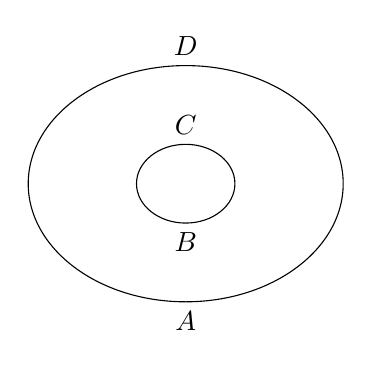
\begin{tikzpicture}
  \draw  circle [x radius = 2.0, y radius = 1.5];
  \draw  circle [x radius = 0.625, y radius = 0.5];
  \node  [below] at (0,-1.5) {$A$};
  \node  [below] at (0,-0.5) {$B$};
  \node  [above] at (0,0.5) {$C$};
  \node  [above] at (0,1.5) {$D$};
\end{tikzpicture}
\end{center}

$a$を正の実数として,$f$の値が$a$以下の部分の図形$T^a$を調べる.図形の様子が変わるのは図の$A$, $B$, $C$, $D$を通るときである.$a$が$f(A)$と$f(B)$の間にあるとき$T^a$はお椀型,すなわち円板$D^2$の形をしている.$f(B)< a< f(C)$のとき,円板$D^2$の境界に$D^1\times D^1$を貼りつけたものが出てくる.$D^1\times D^1$を2次元の1ハンドルという.さらに$a$の値が$C$を超えると,前に貼りつけた1ハンドルの側面にもう一つ1ハンドルをつけた図形が現れる.最後に境界の円周に沿って円板を貼りつけると$T$が復元される.
\end{example}


上の例のように,都合のいい関数をとれば多様体はハンドル$D^\lambda\times D^{n-\lambda}$たちを貼りつけた図形として実現できる.この都合のいい関数はMorse関数とよばれ,豊富に存在することが知られている.このハンドル分解を使って定理\ref{diffeo classification}を示すことができる.

実は,この方法によって微分同相のレベルで閉多様体を分類できることは自明なことではない.ハンドルを貼りつけるという操作をなめらかに行うことができるとは限らないからである.このことは次の二つの事実から分かる.

\begin{fact}[Reebの球面定理]
$n$次元コンパクト多様体$M$上に臨界点を二つしか持たないMorse関数が存在するならば,$M$は$n$次元球面$S^n$と同相である.
\end{fact}

\begin{fact}[Milnorのエキゾチック球面]\label{exotic}
7次元球面$S^7$と同相だが微分同相でない多様体が存在する.
\end{fact}

Reebの球面定理の証明を見ると,$M$は2つの$n$次元円板を貼り合わせた図形になっていることが分かる.このことから$M$と$S^n$が同相であることが分かるが,事実\ref{exotic}はこの貼り合わせががなめらかに行えるとは限らないことを示している.\cite{松本}によると,すべてのハンドルの貼りつけがなめらかに行えるのは6次元以下の多様体に限る.このような特殊事情から2次元閉多様体は微分同相のレベルで分類できる.

\subsection{コンパクトRiemann面の分類}
コンパクトRiemann面は定義から向きづけ可能な2次元閉多様体であるが,これは種数で分類することはできない.実際,種数1のコンパクトRiemann面で互いに双正則同値でないものが非可算個存在することが知られている.一方で種数0のコンパクトRiemann面は$\setC P^1$しかないことが証明できる.

\begin{thebibliography}{99}
\item 小木曽啓示,『代数曲線論』,朝倉書店,2002.
\item 田村一郎,『トポロジー』,岩波書店,1972.
\item 堀川穎二,『新装版 複素代数幾何学入門』,岩波書店,2015.
\item 枡田幹也,『代数的トポロジー』,朝倉書店,2002.
\bibitem{松本} 松本幸夫,『Morse理論の基礎』,岩波書店,1997.
\bibitem{triangle} Doyle, P. H. and Moran, D. A., ``A Short Proof that Compact 2-Manifolds Can Be Triangulated'', \textit{Inventiones math}. \textbf{5}, 160--162, 1968.
\item Francis, G. K. and Weeks, J. R., ``Conway's ZIP Proof'', \textit{Amer. Math. Monthly} \textbf{106}, 393--399, 1999.
\item Hirsch, M. W., \textit{Differential Topology}, Springer, 1976.
\item Milnor, J., \textit{Morse Theory}, Princeton Univ. Press, 1963. 
\bibitem{Seifert} Seifert, H. and Threlfall, W., \textit{A Textbook of Topology}, Academic Press, 1980. 
\end{thebibliography}
\end{document}